\documentclass[14pt]{article}
\usepackage{listings}
\usepackage{color}
\usepackage{graphicx}
\usepackage{setspace}

\definecolor{dkgreen}{rgb}{0,0.6,0}
\definecolor{gray}{rgb}{0.5,0.5,0.5}
\definecolor{mauve}{rgb}{0.58,0,0.82}

\lstset{frame=tb,
  language=java,
  aboveskip=3mm,
  belowskip=3mm,
  showstringspaces=false,
  columns=flexible,
  basicstyle={\small\ttfamily},
  numbers=none,
  numberstyle=\tiny\color{gray},
  keywordstyle=\color{blue},
  commentstyle=\color{dkgreen},
  stringstyle=\color{mauve},
  breaklines=true,
  breakatwhitespace=true
  tabsize=3
}







\begin{document}
\title{% 
  \huge Concurrent and Distributed Systems \\
  \vspace{20mm}
  \large Laboratory Assignment 4 \\}

\date{\today}
\maketitle
\begin{center}
\vspace{30 mm}

\title{\huge Student: Marcu Andrei Cristian}
\\\vspace{10 mm}
\title{\huge Computers and Information Technology}
\\\vspace{10 mm}
\title{\huge CEN 3.2 A}
\\\vspace{10 mm}
\title{\huge 3rd Year}
\end{center}
\date{}
\maketitle

\newpage
\section*{Problems statements}
\vspace{20 mm}
\textbf{Problem 1} (50p) \\
Implement the dining philosophers problem using channels
\\\vspace{10 mm}\\
\textbf{Problem 2} (50p) \\
Implement the readers-writers problem using semaphores
as follows:\\
- More readers can read at the same time the same shared resource as long as
there is no writer with writing access to the same shared resource\\
- A writer will get exclusive access to the shared resource (no other writer and/or reader can have access at the same time to the same shared resource)\\
- There is no starvation for readers or writers
\begin{center}
\end{center}
\newpage
Both problems are implemented using Java.
\\\vspace{10 mm}\\
\textbf{Problem1:} The dining philosophers problem has the next statement. We have n philosophers and n forks around a circular table.Both philosophers and forks are threads. A philosopher needs 2 forks to eat( the left one and the right one ) . Implement a method to synchronize this process. The idea behind the solution is that each philosopher has two adjacent forks. Philosophers communicate with the fork[i] through the channel[i], fork[i+1] through the channel[i+1] etc. Channels are composed of 2 methods ( send and receive ). When a message is RECEIVED it means that the adjacent forks are not in use and the philosopher can pick them up. After the philosopher finishes eating he'll SEND a message to the next philosopher.

\\\vspace{20 mm}\\
\textbf{Problem2:} The readers-writers is a problem like producer consumer. The readers can read only after a writer has finished writing. I've implemented the problem wih 3 semaphores, one for the writer, one for the reader and one which is common for both of them(I've called it orderSemaphore) which keeps the order of the writers and readers, avoiding starvation. I have two methods, read and write. The read method uses all 3 semaphores, the readerSemaphore is acquired and released multiple times so many readers can read at the same time. The order semaphore is acquired to avoid starvation. The writer semaphore is acquired and released when the last reader finished reading. The write method uses the writerSemaphore and orderSemaphore. The writer Semaphore is locked when the writer starts writing and unlocked when it finished. The orderSemaphore is used to avoid starvation.


\newpage
\section*{Source code for Dinning Philosophers with channels}\\
\begin{lstlisting}
//----------------------------Channel.java----------------------------


public class Channel<T> {
	private T chan = null;
	int ready = 0;
	
	public synchronized void send(T mes) throws InterruptedException {
		// save the message in channel
		chan = mes;
		++ready;
		notifyAll();
		while(chan != null) {
			wait();// wait until the message is received, after that the channel becomes null
		}
	}
	
	
	public synchronized T receive() throws InterruptedException {
		
		while(ready == 0) {
			wait();
		}
		--ready;
		T tmp = chan; // we save the message
		chan = null;
		notifyAll();// notify all the senders
		return(tmp);
	}
}	

\end{lstlisting}
\begin{lstlisting}
//----------------------------Fork.java----------------------------

public class Fork extends Thread {

		private Boolean isReceived;
		private int i;
		private ArrayList<Channel<Boolean>> forks;
		
		public Fork(int i, ArrayList<Channel<Boolean>> forks) {
			this.i = i;
			this.forks = forks;
		}
		public void run() {
			
			while(true) {
	
				try {
					(forks.get(i)).send(true);
					isReceived = (forks.get(i)).receive();
				} catch (InterruptedException e) {
					e.printStackTrace();
				}
			}
		}
}

\end{lstlisting}
\begin{lstlisting}
//----------------------------Philosopher.java----------------------------

public class Philosopher extends Thread {
	private Boolean isReceived;
	private String name;
	private int leftFork;
	private int rightFork;
	private ArrayList<Channel<Boolean>> forks;


	public Philosopher(int leftFork, int rightFork, String name, ArrayList<Channel<Boolean>> forks2) {
		this.leftFork = leftFork;
		this.rightFork = rightFork;
		this.forks = forks2;
		this.name = name;
	}

	public void run() {

		while(true) {


			try {
				System.out.println(name + " is thinking");
				Thread.sleep(2000);
				isReceived = (forks.get(leftFork)).receive();
				isReceived = (forks.get(rightFork)).receive();
				System.out.println(name + " is eating");
				Thread.sleep(2000);
				(forks.get(leftFork)).send(true);
				(forks.get(rightFork)).send(true);
			} catch (InterruptedException e) {

				e.printStackTrace();
			}

		}
	}
}

\end{lstlisting}

\begin{lstlisting}
//----------------------------Main.java----------------------------

import java.util.ArrayList;

public class Main {
public static void main(String[] args) throws InterruptedException {
		int philosophersNumber = 5; // no of philosopohers = no of forks
		ArrayList<Channel<Boolean>> forks = new ArrayList<Channel<Boolean>>();
		Fork[] forksArray = new Fork[philosophersNumber];
		Philosopher[] philosophers = new Philosopher[philosophersNumber];
		
		for(int i = 0 ; i < 5 ; ++i) {
			forks.add(new Channel<Boolean>());
		}
						
		
		for (int i = 0; i < philosophersNumber; i++) {
	    	  forksArray[i] = new Fork(i, forks);
	    	  forksArray[i].start();
	    }
		
		for (int i = 0; i < philosophersNumber; i++) {
	        philosophers[i] = new Philosopher(i, (i + 1) % philosophersNumber, "Philo" + i, forks);
	        philosophers[i].start();
	    }
		
		Thread.sleep(5000); // the time is in ms. after this time we stop the execution
		
		
		for(Philosopher philosopher: philosophers)
		{
			philosopher.join();
		}

	}
}

\end{lstlisting}


\vspace{5 mm}\\
\section*{Experiments and results for Dinning Philosophers with channels}
\begin{center}
1. Random example 1 with 5 philosophers and 5 forks\\
\vspace{5mm}
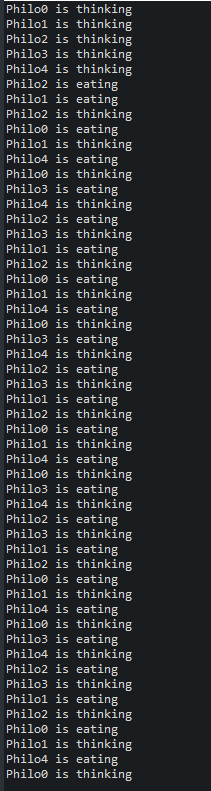
\includegraphics[height=5.5in, width = 1.5in]{philo1.png}\\
\end{center}\\

\begin{center}
2. Random example 2 with 5 philosophers and 5 forks\\
\vspace{5mm}

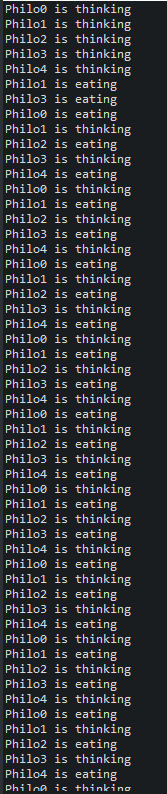
\includegraphics[height=5.5in, width = 1.5in]{philo2.png}\\
\end{center}\\

\begin{center}
\newpage
3. Random example 3 with 4 philosophers and 4 forks\\
\vspace{10mm}

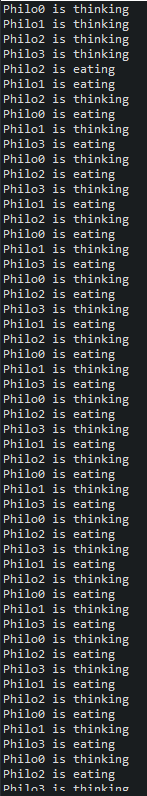
\includegraphics[height=5.5in, width = 1.5in]{philo3.png}\\
\end{center}\\

\section*{Conclusions Producer-Consumer problem}
\vspace{10 mm}
The main problem we need to avoid is the deadlock. Each fork has a synchronization method( doesn't matter if it's a lock/monitor or semaphore because all of them are doing the same thing ). Each fork can be accesed only by one thread at a moment of time, this way two philosophers can't pick the same fork. I've learnt more about deadlocks and concurrent programming synchronization methods

\newpage
\section*{Source code for readers-writers problem with semaphores}\\
\begin{lstlisting}
//----------------------------ReadersWriters.java----------------------------

public class ReadersWriters {
	private int readCount = 0;
	private Semaphore writerSemaphore = new Semaphore(1);
	private Semaphore readerSemaphore = new Semaphore(1);
	private Semaphore orderSemaphore = new Semaphore(1);

	public void write(String writer) {


		// Obtaining access to the resource

		try {
			orderSemaphore.acquire();
			writerSemaphore.acquire();
		} catch (InterruptedException e) {
			e.printStackTrace();
		}

		orderSemaphore.release();

		// Writing into the resource

		try {
			System.out.println(writer + " is writing");
			Thread.sleep(1000);
			System.out.println(writer + " has stopped writing");
		} catch (InterruptedException e) {
			e.printStackTrace();
		}


		writerSemaphore.release();

	}


	public void read(String reader) {

		// Obtaining access to the queue and the readCount variable

		try {
			orderSemaphore.acquire();
			readerSemaphore.acquire();
		} catch (InterruptedException e) {
			e.printStackTrace();
		}


		// First reader obtains access to the resource
		// so that writers are blocked

		if(readCount == 0) {
			try {
				writerSemaphore.acquire();
			} catch (InterruptedException e) {
				e.printStackTrace();
			}
		}

		// Reader starts reading
		readCount++;

		orderSemaphore.release();
		readerSemaphore.release();

		// Reading the resource
		try {
			System.out.println(reader + " is reading");
			Thread.sleep(1000);
			System.out.println(reader + " has stopped reading");
		} catch (InterruptedException e1) {
			e1.printStackTrace();
		}

		// Obtaining access to modify readCount

		try {
			readerSemaphore.acquire();
		} catch (InterruptedException e) {
			e.printStackTrace();
		}

		// Reader stops reading
		readCount--;


		// Releasing access if the current reader is the last reader

		if(readCount == 0) {
			writerSemaphore.release();
		}

		readerSemaphore.release();
	}
}

\end{lstlisting}
\begin{lstlisting}
//----------------------------Reader.java----------------------------

public class Reader extends Thread {
	ReadersWriters rw = new ReadersWriters();
	String name;
	Reader(ReadersWriters rw, String name)
	{
		this.rw = rw;
		this.name = name;
	}
	public void run() {
		for(int i = 0 ; i < 10 ; i++)
		{
			rw.read(name);
		}
    }

}



\end{lstlisting}
\begin{lstlisting}
//----------------------------Writer.java----------------------------


public class Writer extends Thread {
	ReadersWriters rw = new ReadersWriters();
	String name;
	Writer(ReadersWriters rw, String name)
	{
		this.rw = rw;
		this.name = name;
	}
	public void run() {
		for(int i = 0; i < 10; i++)
		{
			rw.write(name);
		}
	}
}

\end{lstlisting}
\begin{lstlisting}
//----------------------------Main.java----------------------------

public class Main {

	public static void main(String[] args) {
		ReadersWriters rw = new ReadersWriters();
		int readersNumber = 2;
		int writersNumber = 1;
		int i;


		Reader[] readers = new Reader[readersNumber + 1];


		// Initializing the readers

		for(i = 1 ; i <= readersNumber ; i++) {
			readers[i] = new Reader(rw, "Reader" + i);
		}

		Writer[] writers = new Writer[writersNumber + 1];


		// Initializing the writers

		for(i = 1 ; i <= writersNumber ; i++) {
			writers[i] = new Writer(rw, "Writer" + i);
		}


		// Starting the threads execution

		for(i = 1 ; i <= writersNumber ; i++) {
			writers[i].start();
		}
		
		for(i = 1 ; i <= readersNumber ; i++) {
			readers[i].start();
		}


		for(i = 1 ; i <= readersNumber ; i++) {
			try {
				readers[i].join();
			} catch (InterruptedException e) {
				e.printStackTrace();
			}
		}

		for(i = 1 ; i <= writersNumber ; i++) {
			try {
				writers[i].join();
			} catch (InterruptedException e) {
				e.printStackTrace();
			}
		}

	}

}



\end{lstlisting}
\newpage{}
\section*{Experiments and results for readers-writers with semaphores}
\\\\\\
\begin{center}
Both the writers and readers will do 10 steps.\\
1. Random example 1 with 2 readers 1 writer\\
\vspace{10mm}

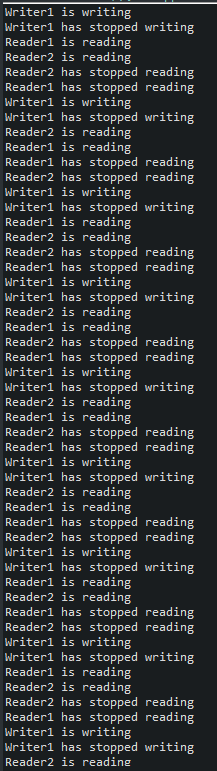
\includegraphics[height=5.5in, width = 2.5in]{rw1.png}\\
\end{center}\\
\newpage{}
\begin{center}
2. Random example 2 with 3 readers 2 writers\\
\vspace{10mm}

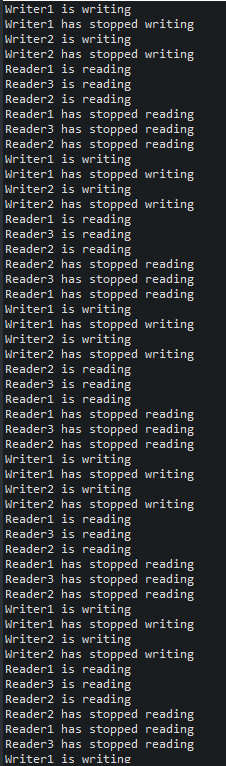
\includegraphics[height=5.5in, width = 2.5in]{rw2.png}\\
\end{center}\\
\newpage{}
\begin{center}
3. Random example 3 with 5 readers 2 writers\\
\vspace{10mm}

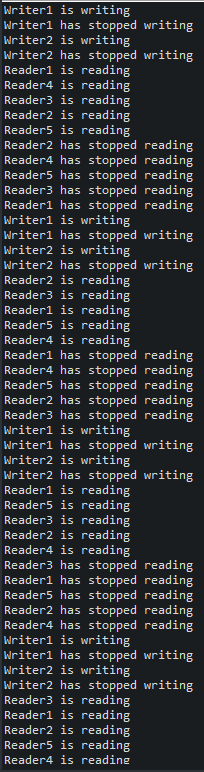
\includegraphics[height=5.5in, width = 2.5in]{rw3.png}\\
\end{center}\\


\section*{Conclusions Readers Writers problem}
\vspace{10 mm}
Working on the readers-writers problem I've learnt more about semaphores and starvation. 

\newpage
\section*{References}
https://en.wikipedia.org/wiki/Readers%E2%80%93writers_problem

\end{document}